\documentclass[aspectratio=1610,slidestop]{beamer}

\author{Mihai Lefter}
\title{Python Programming}
\providecommand{\mySubTitle}{Introduction}
\providecommand{\myConference}{Programming Course}
\providecommand{\myDate}{26-11-2018}
\providecommand{\myGroup}{}
\providecommand{\myDepartment}{}
\providecommand{\myCenter}{}

\usetheme{lumc}

\usepackage{minted}
\usepackage{tikz}
\usepackage[many]{tcolorbox}

\definecolor{monokaibg}{HTML}{272822}
\definecolor{emailc}{HTML}{1e90FF}
\definecolor{scriptback}{HTML}{CDECF0}
\definecolor{ipyout}{HTML}{F0FFF0}

\newenvironment{ipython}
 {\begin{tcolorbox}[title=IPython,
                   title filled=false,
                   fonttitle=\scriptsize,
                   fontupper=\footnotesize,
                   enhanced,
                   colback=monokaibg,
                   drop small lifted shadow,
                   boxrule=0.1mm,
                   left=0.1cm,
                   arc=0mm,
                   colframe=black]}
 {\end{tcolorbox}}



\newenvironment{terminal}
 {\begin{tcolorbox}[title=terminal,
                   title filled=false,
                   fonttitle=\scriptsize,
                   fontupper=\footnotesize,
                   enhanced,
                   colback=monokaibg,
                   drop small lifted shadow,
                   boxrule=0.1mm,
                   left=0.1cm,
                   arc=0mm,
                   colframe=black]}
 {\end{tcolorbox}}


\newcommand{\hrefcc}[2]{\textcolor{#1}{\href{#2}{#2}}}
\newcommand{\hrefc}[3]{\textcolor{#1}{\href{#2}{#3}}}

\newcounter{cntr}
\renewcommand{\thecntr}{\texttt{[\arabic{cntr}]}}

\newenvironment{pythonin}[1]
{\VerbatimEnvironment
  \begin{minipage}[t]{0.11\linewidth}
   \textcolor{green}{\texttt{{\refstepcounter{cntr}In \thecntr:}}}
  \end{minipage}%
  \begin{minipage}[t]{0.89\linewidth}%
  \begin{minted}[
    breaklines=true,style=monokai]{#1}}
 {\end{minted}
 \end{minipage}}

\newenvironment{pythonout}
{%
  \addtocounter{cntr}{-1}
  \begin{minipage}[t]{0.11\linewidth}
   \textcolor{red}{\texttt{{\refstepcounter{cntr}Out\thecntr:}}}
  \end{minipage}%
  \color{ipyout}%
  \ttfamily%
  \begin{minipage}[t]{0.89\linewidth}%
}
{\end{minipage}}

\newenvironment{pythonerr}[1]
{\VerbatimEnvironment
  \begin{minted}[
    breaklines=true,style=monokai]{#1}}
 {\end{minted}}


\newenvironment{pythonfile}[1]
 {\begin{tcolorbox}[title=#1,
                    title filled=false,
                    coltitle=LUMCDonkerblauw,
                    fonttitle=\scriptsize,
                    fontupper=\footnotesize,
                    enhanced,
                    drop small lifted shadow,
                    boxrule=0.1mm,
                    leftrule=5mm,
                    rulecolor=white,
                    left=0.1cm,
                    colback=white!92!black,
                    colframe=scriptback]}
 {\end{tcolorbox}}


\newenvironment{pythoncode}
 {\begin{tcolorbox}[title filled=false,
                    coltitle=LUMCDonkerblauw,
                    fonttitle=\scriptsize,
                    fontupper=\footnotesize,
                    enhanced,
                    drop small lifted shadow,
                    boxrule=0.1mm,
                    leftrule=5mm,
                    rulecolor=white,
                    left=0.1cm,
                    colback=white!92!black,
                    colframe=scriptback]}
 {\end{tcolorbox}}


\newenvironment{pythonoutnonumber}
{%
  \color{ipyout}%
  \ttfamily%
}
{}


\usepackage[inkscapelatex=false]{svg}

\begin{document}

% This disables the \pause command, handy in the editing phase.
%\renewcommand{\pause}{}

% Make the title slide.
\makeTitleSlide{\includesvg[height=3.5cm]{../../images/Python.svg}}



% First page of the presentation.
\section{Introduction}
\makeTableOfContents

\subsection{Why Python?}
\begin{pframe}
 \vspace{-0.3cm}
 \begin{itemize}
  \item Widely used with a large community.
 \end{itemize}
 \vspace{-0.5cm}
 \begin{center}
  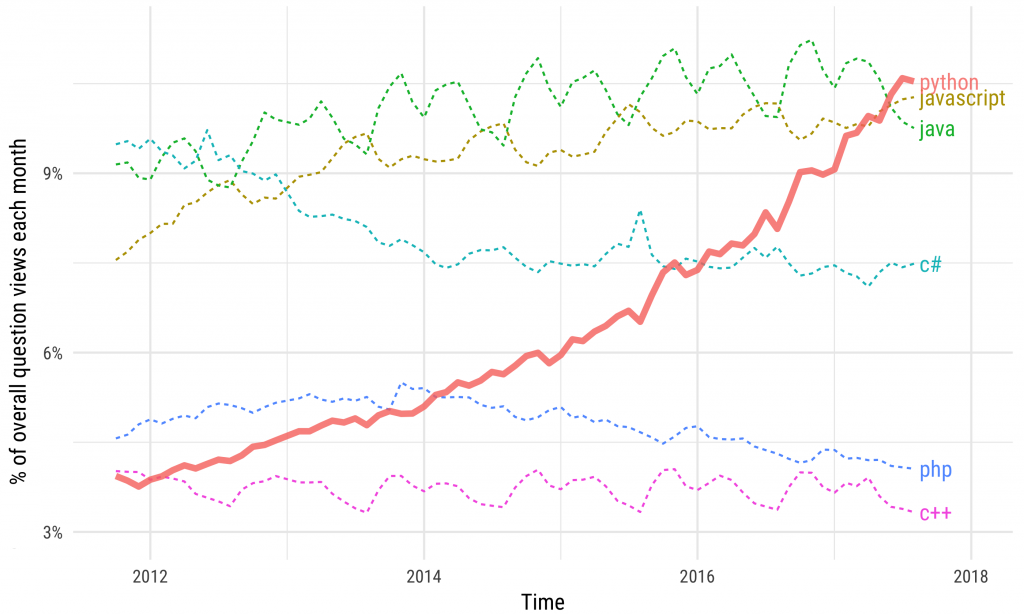
\includegraphics[width=0.72\textwidth]{../../images/growth_major_languages-1-1024x878_stackoverflow_c.png}
  \tiny{https://stackoverflow.blog/2017/09/06/incredible-growth-python/}
 \end{center}
\end{pframe}

\begin{pframe}
 \vspace{-0.3cm}
 \begin{itemize}
  \item Widely used with a large community.
 \end{itemize}
 \vspace{-0.5cm}
 \begin{center}
  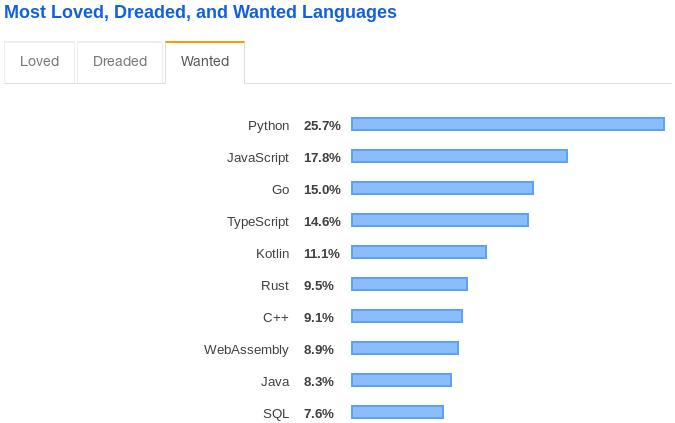
\includegraphics[width=0.70\textwidth]{../../images/stackoverflow_most_wanted_2019.png}\\
  \tiny{https://insights.stackoverflow.com/survey/2019/\#most-loved-dreaded-and-wanted}
 \end{center}
\end{pframe}

\begin{pframe}
 \vspace{-0.3cm}
 \begin{itemize}
  \item Widely used with a large community.
 \end{itemize}
 \vspace{-0.5cm}
 \begin{center}
  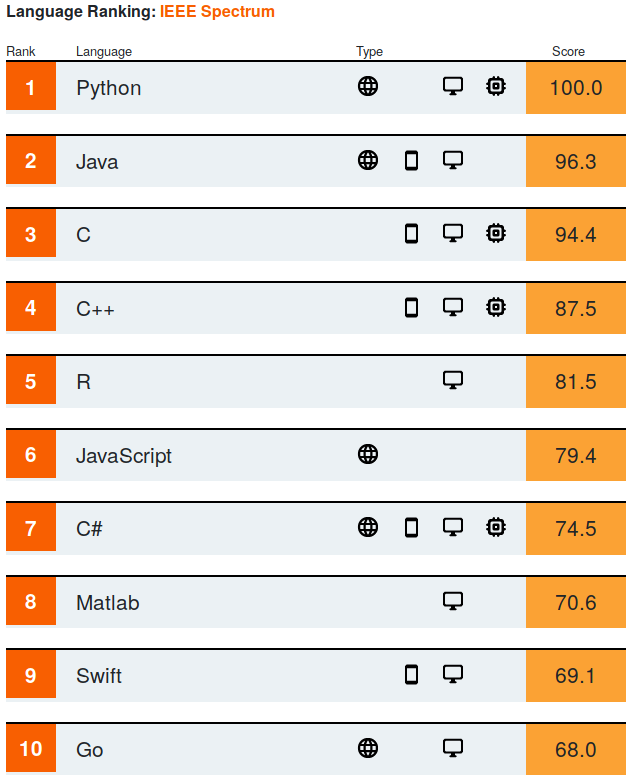
\includegraphics[width=0.35\textwidth]{../../images/ieee_programming_languages_top_2019.png}\\
  \tiny{https://spectrum.ieee.org/computing/software/the-top-programming-languages-2019}
 \end{center}
\end{pframe}

\begin{pframe}
 \begin{tikzpicture}[remember picture,overlay]
    \node[xshift=-4.5cm,yshift=-6.5cm] at (current page.north east)
    {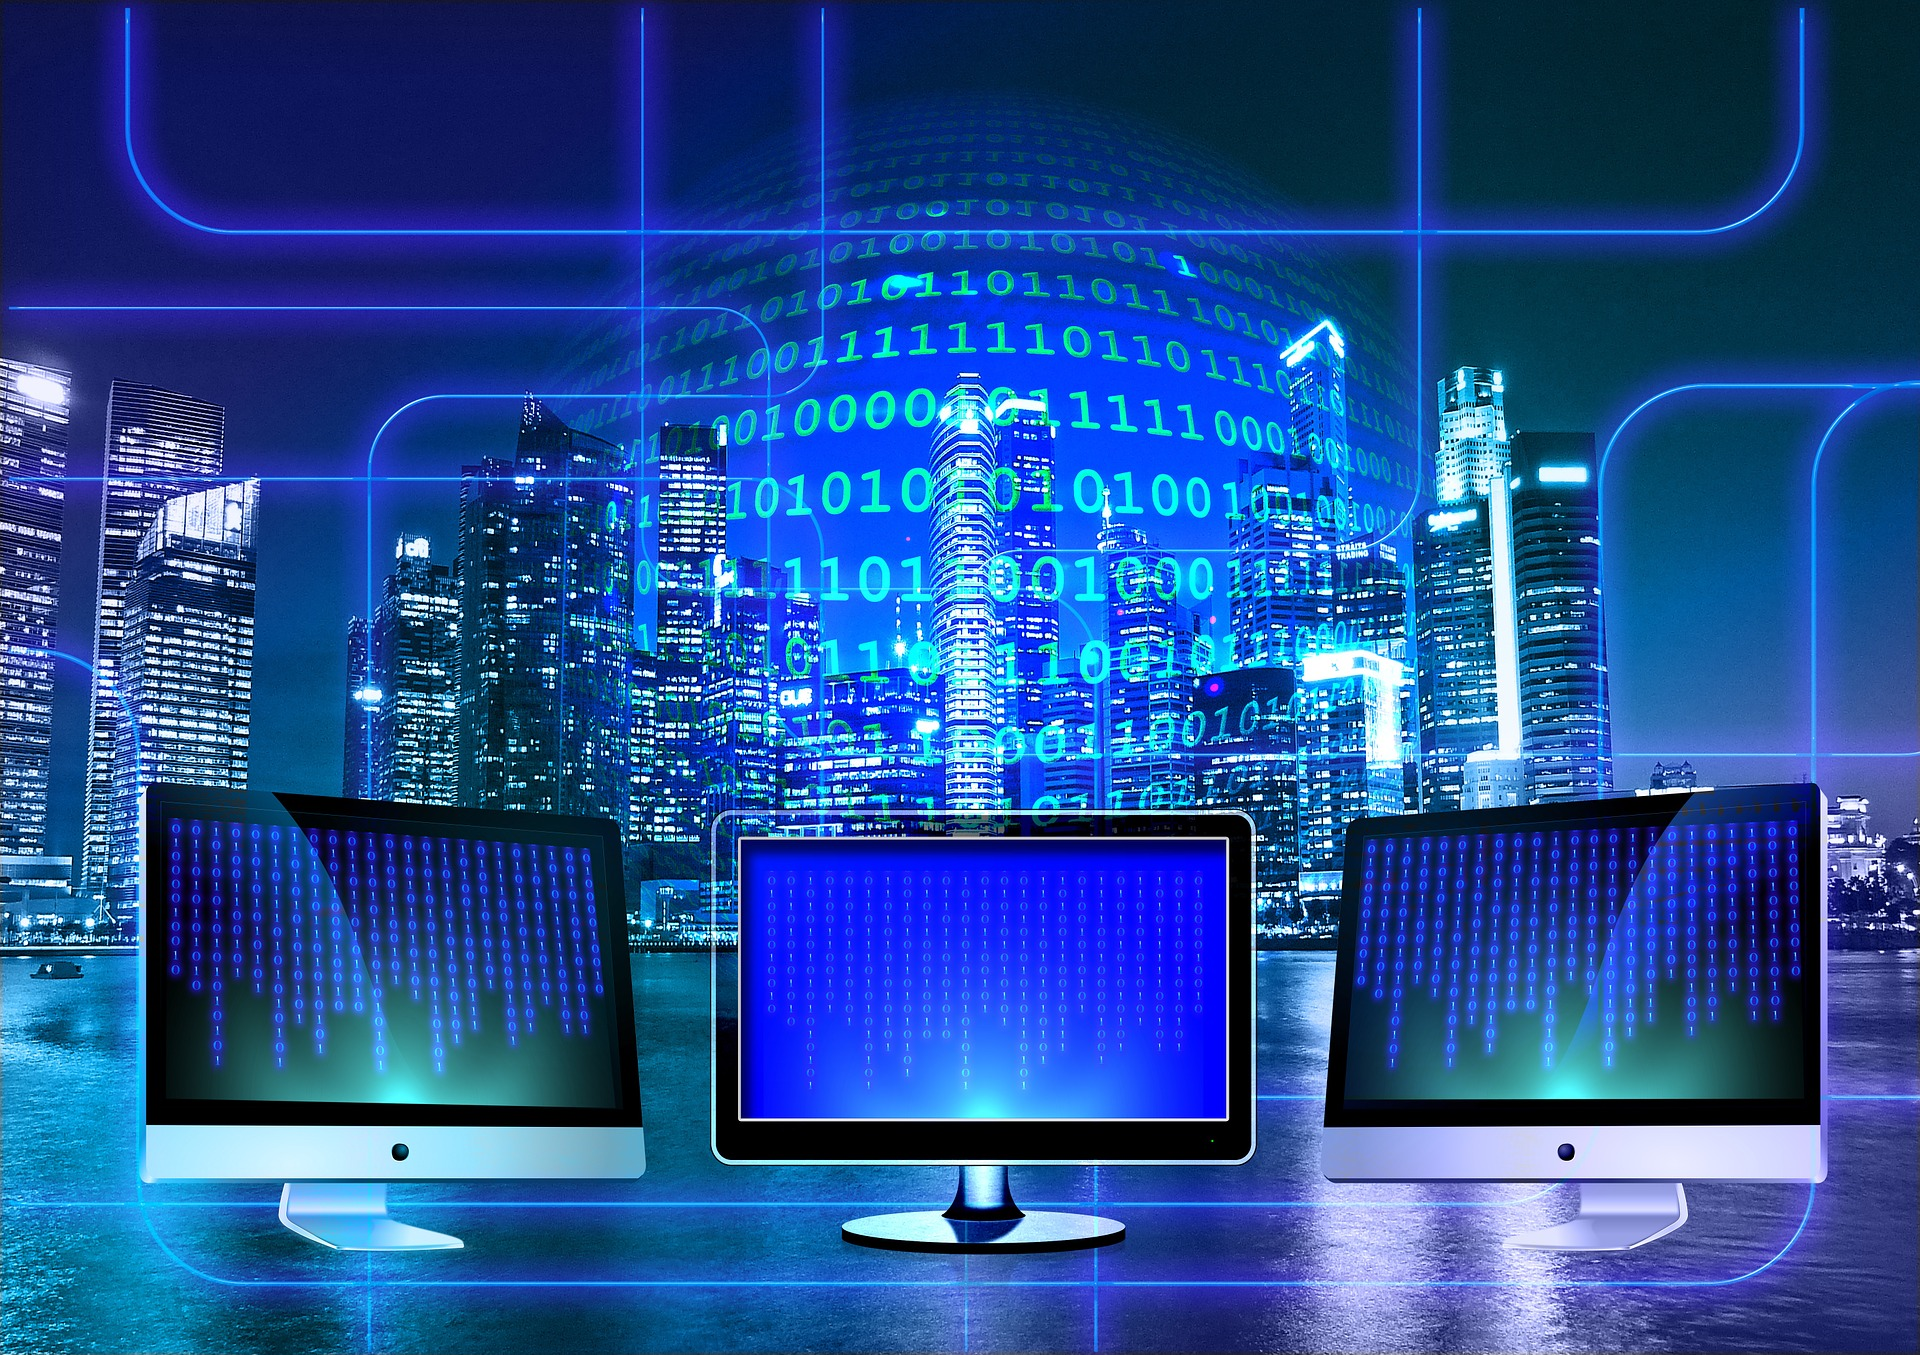
\includegraphics[width=6cm]{../../images/widely.jpg}};
  \end{tikzpicture}
 \begin{itemize}
  \item Widely used with a large community.
  \item Rich (scientific) libraries.
  \item Low barrier to entry.
 \end{itemize}
\end{pframe}


\section{About Python}

\subsection{History}
\begin{pframe}
 \begin{itemize}
  \item Created early 90's by Guido van Rossem at CWI.
  \begin{itemize}
   \item Name: Monty Python.
  \end{itemize}
  \item Design is driven by code readability.
 \end{itemize}
 \begin{tikzpicture}[remember picture,overlay]
   \node[xshift=-4.5cm,yshift=-6.5cm] at (current page.north east)
   {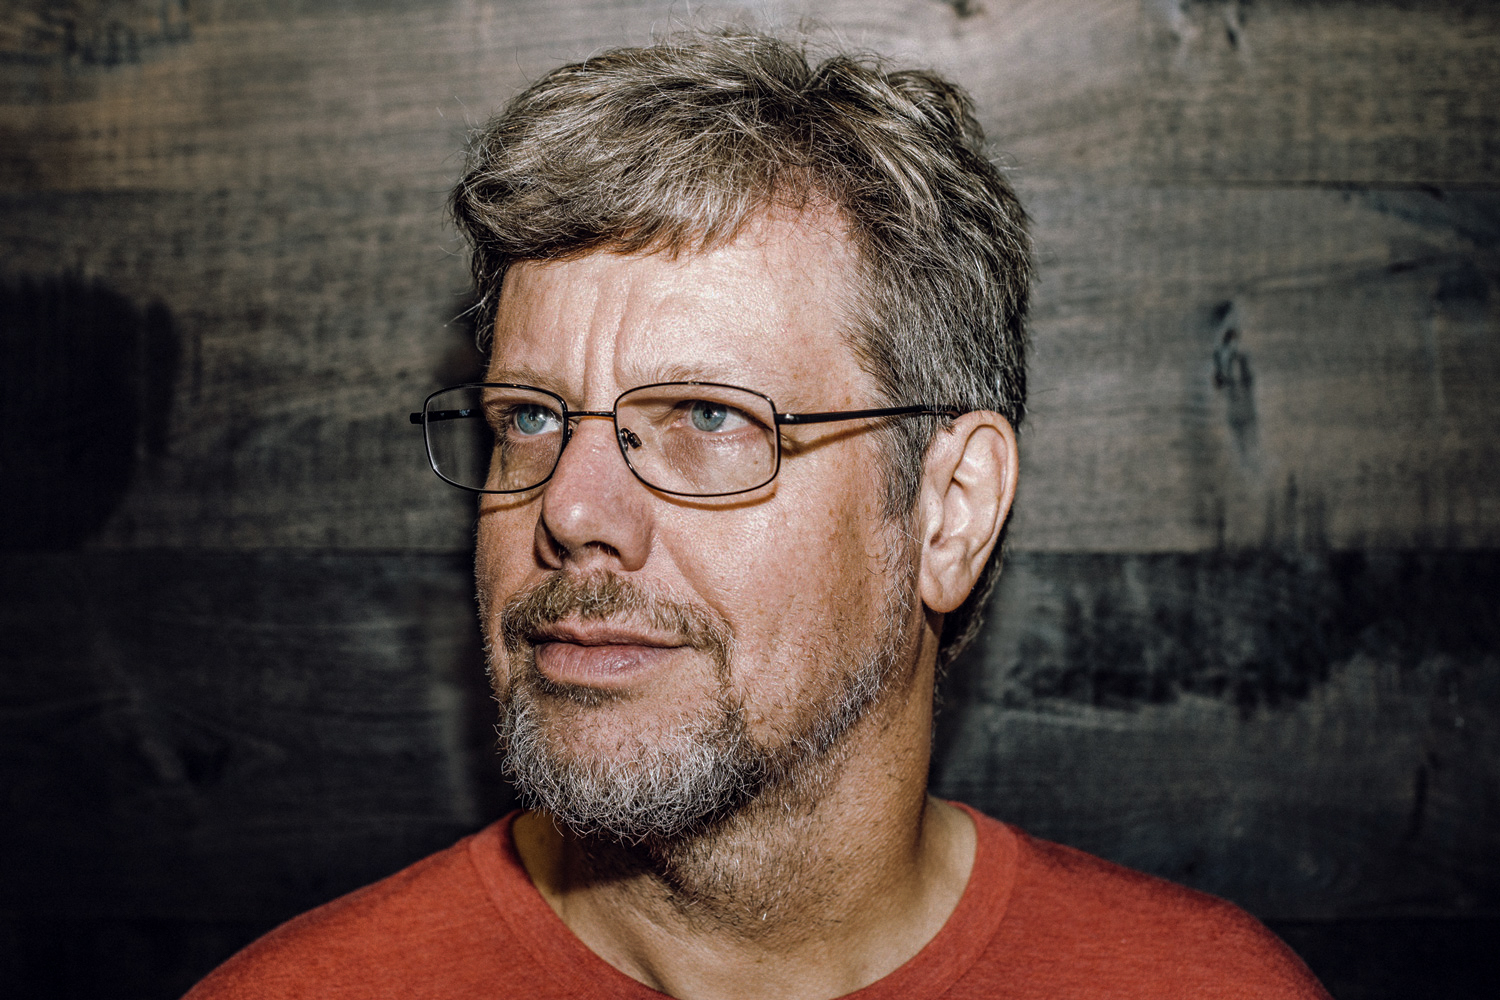
\includegraphics[width=6cm]{../../images/Guido.jpg}};
 \end{tikzpicture}
 \begin{tikzpicture}[remember picture,overlay]
   \node[xshift=-11.5cm,yshift=-6.5cm] at (current page.north east)
   {\includesvg[width=6cm]{../../images/cwi.svg}};
 \end{tikzpicture}
\end{pframe}

\subsection{Python 2 versus Python 3}
\begin{pframe}
 \begin{itemize}
  \item Python 2.7 is the last Python 2.
  \item Python 3 is backwards incompatible.
  \item Some libraries don't support it yet.
  \item Some Python 3 features are backported in Python 2.7.
  \item Last Python 2 release in April 2020.
 \end{itemize}
  We'll use Python 3 for this course.
\end{pframe}

\subsection{Features}
\begin{pframe}
 \begin{tikzpicture}[remember picture,overlay]
  \node[xshift=-4.5cm,yshift=-6.7cm] at (current page.north east)
  {
\includegraphics[width=6cm]{../../images/abstract.jpg}};
 \end{tikzpicture}
 \begin{itemize}
  \item General purpose, high-level programming language.
  \pause
  \item Interpreted, no separate compilation step needed.
  \pause
  \item Imperative and object-oriented programming.
  \begin{itemize}
   \item And some functional programming.
  \end{itemize}
  \pause
  \item Dynamic type system.
  \pause
  \item Automatic memory management.
 \end{itemize}
\end{pframe}

\section{Running Python Code}
\begin{pframe}
\vspace{-0.5cm}
\begin{minipage}[t]{0.47\textwidth}
  Interactively:
  {\small
  \begin{itemize}
    \item Statement by statement, directly in the interpreter.
  \end{itemize}}
  \pause
  \begin{terminal}
  {\tiny \color{white}{
   \begin{lstlisting}[frame=,style=,numbers=none,aboveskip=-0.1cm,belowskip=-0.1cm]
$ python
Python 3.7 (default, Nov 26 2019, 10:23:46)
[GCC 5.4.0 20160609] on linux
Type "help", "copyright", "credits" or
"license" for more information.
>>> print('Hello world')
Hello world
>>>
  \end{lstlisting}}}
 \end{terminal}
 \pause
 {\small
 \begin{itemize}
  \item Interpreters are great for prototyping.
  \item But not really suitable if you want to share or release code.
 \end{itemize}}
 \end{minipage}\qquad%
 \begin{minipage}[t]{0.47\textwidth}
  \pause
  \vspace{-0.3cm}
  Non-interactively:
  {\small
  \begin{itemize}
   \item By editing a file and running the code afterwards.
  \end{itemize}}
  \pause
  \begin{pythonfile}{first\_script.py}
   \begin{minted}[linenos]{python}
print("Hello world!")
   \end{minted}
  \end{pythonfile}
  \pause
  \begin{terminal}
   {\tiny \color{white}{
   \begin{lstlisting}[frame=,style=,numbers=none,aboveskip=-0.1cm,belowskip=-0.1cm]
$ python first_script.py
Hello world
$
   \end{lstlisting}}}
  \end{terminal}
 \end{minipage}
\end{pframe}


\section{This Course}
\begin{pframe}
 \begin{itemize}
  \item Aimed at PhD students, Postdocs, researchers, analysts, ...
  \item Focus on:
  \begin{itemize}
   \item Programming as a tool to do your research.
   \item Basic understanding of Python.
  \end{itemize}
 \end{itemize}
 \medskip

 \begin{minipage}{0.47\textwidth}
 \begin{center}
   
\includegraphics[width=0.69\textwidth]{../../images/laptop_man.jpg}
 \end{center}
 \end{minipage}%
 \begin{minipage}{0.47\textwidth}
 \begin{center}
   
\includegraphics[width=0.9\textwidth]{../../images/dna.jpg}
 \end{center}
 \end{minipage}
\end{pframe}

\subsection{Hands On!}
\begin{pframe}
 Programming is fun!
 \begin{itemize}
  \item You only learn programming by doing it.
  \item Lecture format:
  \begin{itemize}
   \item Blended teaching + exercising.
  \end{itemize}
  \item Repeat the code from the slides/ \\
  lectures and play around with it.
  \item Do the session exercises.
  \item Practical sessions.
 \end{itemize}
 \begin{tikzpicture}[remember picture,overlay]
    \node[xshift=-4.5cm,yshift=-6.5cm] at (current page.north east)
    {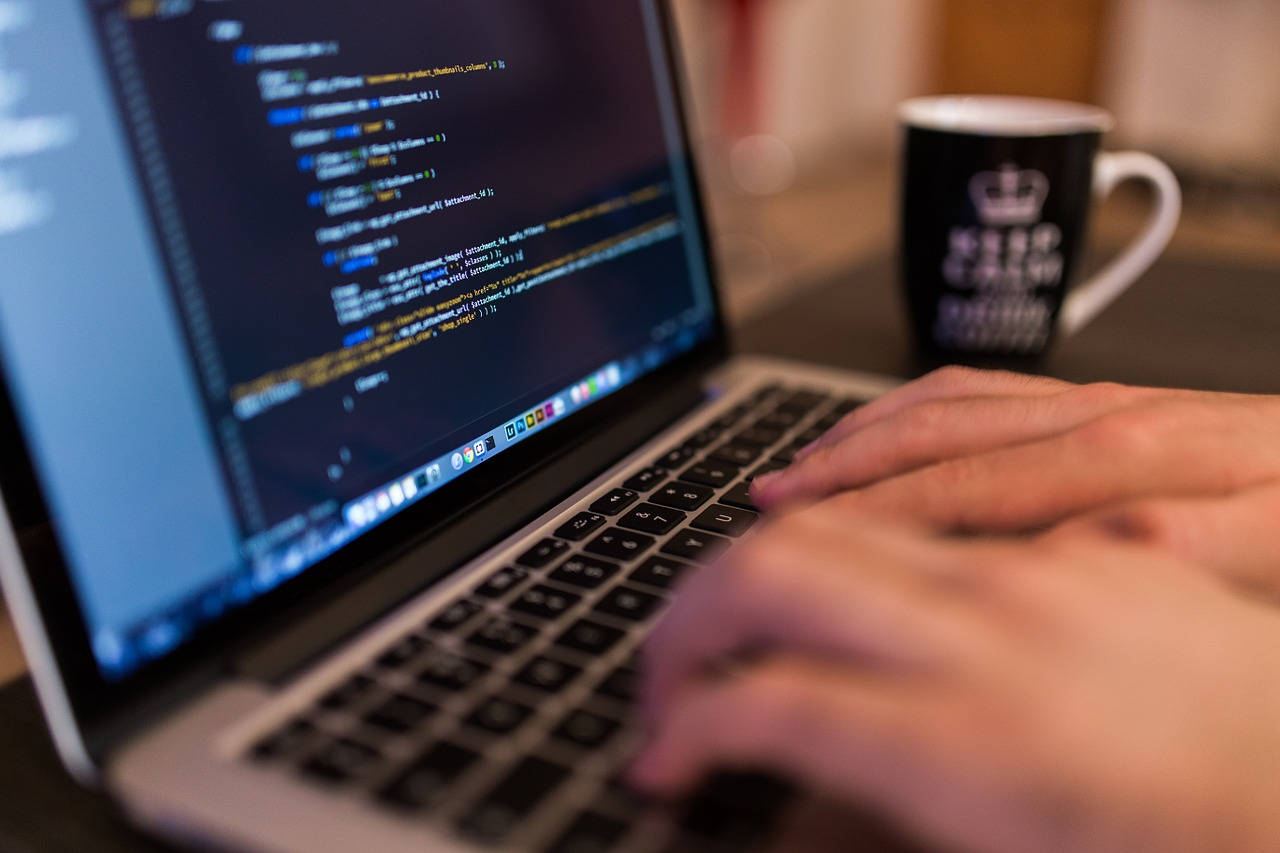
\includegraphics[width=6cm]{../../images/hands_on.jpg}};
  \end{tikzpicture}
\end{pframe}

\subsection{Program}
\begin{pframe}
 \begin{center}
  \includesvg[width=\textwidth]{../../images/program_2020.svg}
 \end{center}
\end{pframe}

\subsection{Material}
\begin{pframe}
 \hrefcc{emailc}{https://github.com/LUMC/python-course}

 \begin{center}
   
\includegraphics[width=0.95\textwidth]{../../images/books.jpg}
 \end{center}
\end{pframe}

\subsection{Practical Sessions}
\begin{pframe}
 \begin{itemize}
  \item We make use of GitHub Classroom.
  \begin{itemize}
   \item GitHub account required.
   \item Receive link with assignment repository.
  \end{itemize}
  \item Own forked repository to work on:
  \begin{itemize}
   \item Clone it.
   \item Code it.
   \item Push it.
  \end{itemize}
  \item Direct file upload to repository\\
  is also possible.
 \end{itemize}
 \begin{tikzpicture}[remember picture,overlay]
    \node[xshift=-4.5cm,yshift=-6.3cm] at (current page.north east)
    {
\includegraphics[width=6cm]{../../images/assignments.jpg}};
  \end{tikzpicture}
\end{pframe}

\subsection{Software requirements}
\begin{pframe}
 \begin{itemize}
  \item Anaconda:
  \begin{itemize}
   \item Python $3.x$.
   \item Comes with all that's required:
   \begin{itemize}
    \item Python interpreter.
    \item Jupyter Notebook.
    \item Libraries: NumPy, Panda,\\
    matplotlib, Bokeh, Biopython, ...
   \end{itemize}
   \item \hrefc{emailc}{http://docs.anaconda.com/anaconda/install/}{Installation instructions}.
  \end{itemize}
  \bigskip
  \item Git:
  \begin{itemize}
   \item \hrefc{emailc}{https://git-scm.com/book/en/v2/Getting-Started-Installing-Git}{Installation instructions}.
  \end{itemize}
 \end{itemize}
 \begin{tikzpicture}[remember picture,overlay]
  \node[xshift=-4.5cm,yshift=-5.5cm] at (current page.north east)
  {\includesvg[width=3cm]{../../images/requirements_logos.svg}};
 \end{tikzpicture}
\end{pframe}

\subsection{Getting help}
\begin{pframe}
 \begin{itemize}
  \item Ask a question.
 \end{itemize}
 \begin{center}
  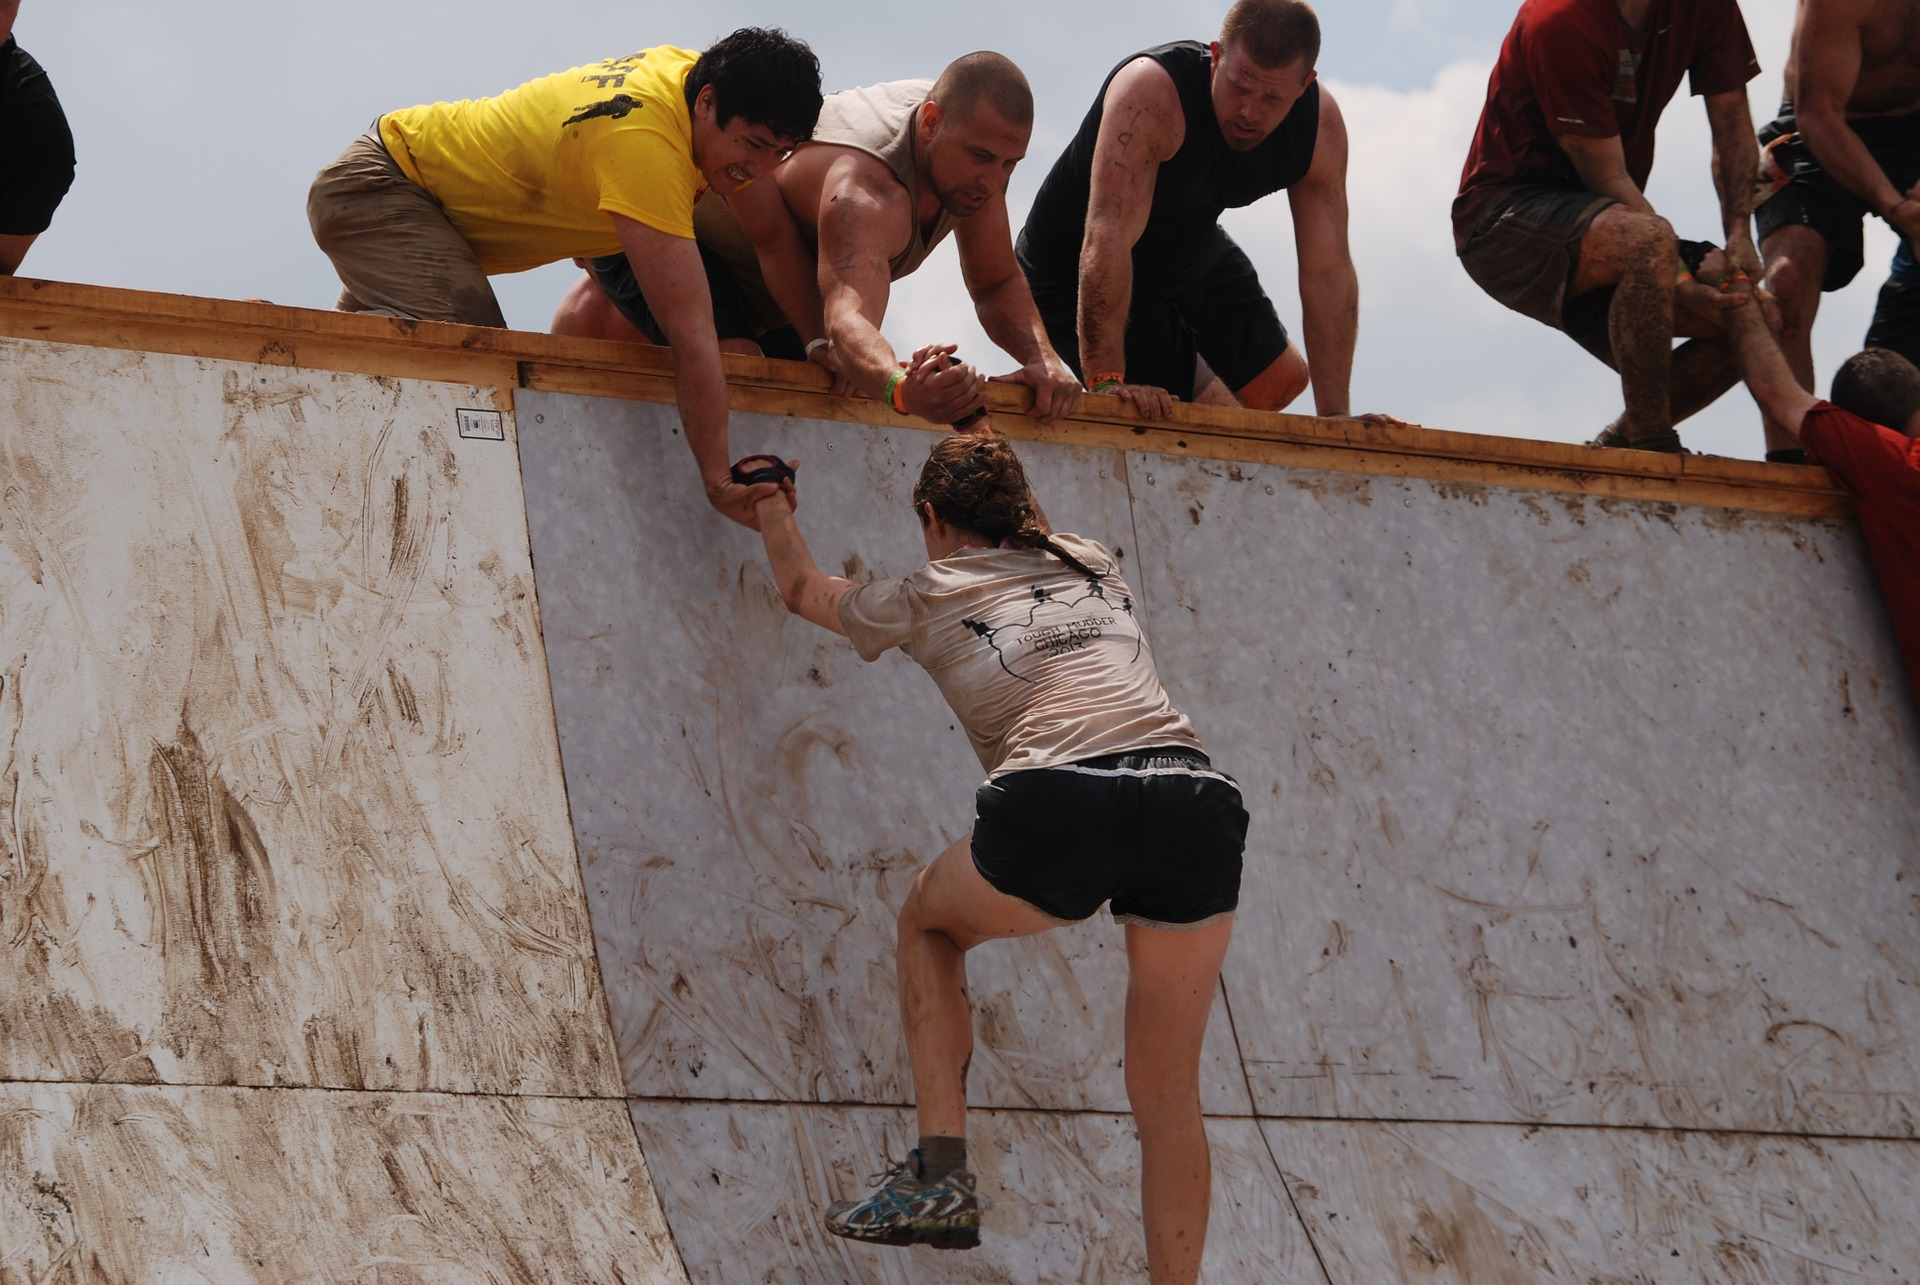
\includegraphics[width=0.54\textwidth]{../../images/help.jpg}
 \end{center}
\end{pframe}

\subsection{Teachers}
\begin{pframe}
 \begin{minipage}[t]{0.5\textwidth}
  \begin{itemize}
   \item Mark Santcroos \\
     \hrefcc{emailc}{m.a.santcroos@lumc.nl}
   \item Ruben Vorderman \\
     \hrefcc{emailc}{r.h.p.vorderman@lumc.nl}
   \item Redmar van den Berg \\
     \hrefcc{emailc}{r.r.van\_den\_berg@lumc.nl}
   \item Mihai Lefter\\
    \hrefcc{emailc}{m.lefter@lumc.nl}
  \end{itemize}
 \end{minipage}
  \begin{tikzpicture}[remember picture,overlay]
    \node[xshift=-5.0cm,yshift=-6.0cm] at (current page.north east)
    {\includesvg[width=7cm]{../../images/class.svg}};
  \end{tikzpicture}
\end{pframe}



% Make the acknowledgements slide.
\makeAcknowledgementsSlide{
  \begin{tabular}{ll}
    Martijn Vermaat\\
    Jeroen Laros\\
    Jonathan Vis
  \end{tabular}
}

\end{document}
